\documentclass[mathserif, xcolor=table]{beamer}

\usepackage[utf8]{inputenc}
\usepackage{graphicx}
\usepackage{mathtools}
\usepackage{amsthm}
\usepackage{algorithmic}
\usepackage{booktabs}

%\addbibresource{references.bib}

\usepackage{hyperref}

\hypersetup{
	colorlinks=true,
	linkcolor=darkred,
	filecolor=darkred,      
	urlcolor=darkred,
}

\usepackage{pgfplots}
\pgfplotsset{compat=1.16}
\usepgfplotslibrary{colorbrewer}


\pgfplotsset{every axis/.append style={
            		width=2.5in,
            		grid=both,
                    label style={font=\footnotesize},
                    tick label style={font=\footnotesize},
            		cycle list/Set1-5,
            		cycle multiindex* list={
            		    Set1-5
            		    \nextlist
                        marks
                        \nextlist
                        [2 of]linestyles
                        \nextlist
            		    thick
            		    \nextlist
                    },
            }
}

\pgfplotsset{
    % define a `cycle list' for marker
    cycle list/.define={marks}{
	    every mark/.append style={solid,fill opacity=0.25,fill=\pgfkeysvalueof{/pgfplots/mark list fill}},mark=*\\
	    every mark/.append style={solid,fill opacity=0.25,fill=\pgfkeysvalueof{/pgfplots/mark list fill}},mark=square*\\
	    every mark/.append style={solid,fill opacity=0.25,fill=\pgfkeysvalueof{/pgfplots/mark list fill}},mark=triangle*\\
	    every mark/.append style={solid,fill opacity=0.25,fill=\pgfkeysvalueof{/pgfplots/mark list fill}},mark=diamond*\\
    },
}


\usetheme{default}
\usecolortheme{beaver}

\title{Iteration for Contour-Based\\ Nonlinear Eigensolvers}
\author{Julien Brenneck \and Eric Polizzi}
\institute[shortist]{UMass Amherst, Department of Mathematics and Statistics}
\date{}
%\subject{Numerical Linear Algebra}

\beamertemplatenavigationsymbolsempty{}

%%%%%%%%%%%%%%%%%%%%%%%%%%%%%%%%%%%%%%%%%%%%%%%%%%%%%%%%%%%%%%%%%%%%%%%%%%%%%%%%
%%%%%%%%%%%%%%%%%%%%%%%%%%%%%%%%%%%%%%%%%%%%%%%%%%%%%%%%%%%%%%%%%%%%%%%%%%%%%%%%
%%%%%%%%%%%%%%%%%%%%%%%%%%%%%%%%%%%%%%%%%%%%%%%%%%%%%%%%%%%%%%%%%%%%%%%%%%%%%%%%

\begin{document}

\begin{frame}
 \titlepage{}
 \nocite{*}
\end{frame}

%%%%%%%%%%%%%%%%%%%%%%%%%%%%%%%%%%%%%%%%%%%%%%%%%%%%%%%%%%%%%%%%%%%%%%%%%%%%%%%%
\section{Background}
%%%%%%%%%%%%%%%%%%%%%%%%%%%%%%%%%%%%%%%%%%%%%%%%%%%%%%%%%%%%%%%%%%%%%%%%%%%%%%%%

\begin{frame}{The Nonlinear Eigenvalue Problem}
	Working towards a ``black box'' solver for the nonlinear eigenvalue problem for matrix valued functions \( T \in H(\Omega, \mathbb{C}^{n\times n}) \).
	\vspace{1em}
	\begin{equation}
		T(\lambda)x = 0,
		\quad\quad x \in \mathbb{C}^n,
		\quad\quad \lambda \in \mathbb{C}
	\end{equation}

	\vspace{1.5em}
	Here \( T(\lambda) = A-\lambda I \) recovers the standard eigenvalue problem.

	\vspace{3em}
	See the review paper by G\"uttel and Tisseur \cite{guttel2017}~for an overview.
\end{frame}


%%%%%%%%%%%%%%%%%%%%%%%%%%%%%%%%%%%%%%%%%%%%%%%%%%%%%%%%%%%%%%%%%%%%%%%%%%%%%%%%
\section{Previous Techniques}
%%%%%%%%%%%%%%%%%%%%%%%%%%%%%%%%%%%%%%%%%%%%%%%%%%%%%%%%%%%%%%%%%%%%%%%%%%%%%%%%

\begin{frame}{Previous Techniques}
	Contour based methods:
	\begin{itemize}
		\item Beyn's method
		\item SS methods of Yokota, Sakurai, Asakura, et al.
		\item NLFEAST
	\end{itemize}
	
	\vspace{1em}

	Newton and Approximation based methods:
	\begin{itemize}
		\item Newton methods, such as residual inverse iteration (RII)
		\item Infinite Arnoldi, Krylov methods
		\item NLEIGS, CORK
		\item Many others
	\end{itemize}
	
\end{frame}

\begin{frame}{Contour}
	Example contour for Butterfly problem (quartic).
    \begin{figure}[htbp]
            \centering
            \begin{tikzpicture}[scale=1.4]
            \begin{axis}[
                    xlabel={Real},
                    ylabel={Imaginary},
                    xmin=0,
		    xticklabels={},
		    yticklabels={},
                    xmax=2,
                    ymin=0,
                    ymax=2]
                    \draw [dashed, thick] (axis cs:1.0,1.0) circle [radius=0.5];
                    \addplot+ [only marks] table {bf_eig_in.dat};
                    \addplot+ [only marks, mark=*, mark options={solid, scale=0.35}] table {bf_eig.dat};
		    \addplot [domain=2*pi/16:2*15*pi/16, samples = 8, only marks] ({0.5*cos(deg(x))+1}, {0.5*sin(deg(x))+1});
            \end{axis}
            \end{tikzpicture}
    \end{figure}
\end{frame}


\begin{frame}{Beyn's Method}

	\begin{equation}
		\frac{1}{2 \pi i} \int_\Gamma f(z) {T(z)}^{-1} \, dz = V f(J) W^H 
	\end{equation}

	Use the Keldysh theorem to probe Jordan decomposition of \( T(\lambda) \) locally in a contour for spectral information. Approximate moments
	\begin{align}
		A_k = \frac{1}{2 \pi i} \int_\Gamma z^k {T(z)}^{-1} X \, dz
		= V \Lambda^k W^H X.
	\end{align}
	With ``probing matrix'' \( X \). In particular,
	\begin{align}
		A_0 = VW^H X,
		&&
		A_1 = V \Lambda W^H X.
	\end{align}

	\vspace{1em}	

	Computing a decomposition of \( A_0 \) and applying a similarity transform, we can compute \( V, \Lambda \) from \( A_0 \) and \( A_1 \).
	
	\vspace{1em}


	%Taking the SVD \( A_0 = V_0 \Sigma_0 W_0^H \) we can derive the following (computable) similarity.
	%\begin{align}
		%\Lambda \sim V_0^H A_1 W_0 \Sigma_0^{-1}
	%\end{align}
	%This gives a standard problem \(  V_0^H A_1 W_0 \Sigma_0^{-1} Y = Y \Lambda\), taking \( X = V_0 Y  \) recovers eigenvectors.

\end{frame}

\begin{frame}{Beyn's Method}
	Pros
	\begin{itemize}
		\item Any type of nonlinearity in \( T(\lambda) \) (no need for approximation).
		\item Highly parallel.
		\item Spectral slicing.
		\item Generalizes to higher moments.
		\item Converges in number of quadrature nodes.
	\end{itemize}
	
	\vspace{1.5em}

	Cons
	\begin{itemize}
		\item Many linear system solves needed (main computational cost).
		\item Linear systems need to be solved accurately.
		\item No way to iterate (other than adaptive quadrature).
		\item For many contour nodes, can be difficult to position away from eigenvalues.
	\end{itemize}
\end{frame}

\begin{frame}{NLFEAST}

	Applying a Residual Inverse Iteration with contour points as fixed shifts gives a Newton-type iteration. 

	\begin{align}
		Q_0 = \frac{1}{2 \pi i } \int_\Gamma \Big(X - {T(z)}^{-1} T(X, \Lambda) \Big) {(zI - \Lambda)}^{-1} \, dz
	\end{align}
	
	\vspace{2em}

	Each iteration we solve the projected nonlinear reduced problem.

	\begin{align}
		Q_0^H T(\lambda) Q_0 y = 0
	\end{align}


	%NLFEAST is in general a projection method. For polynomial problems the reduced system can be solved by companion problem, making it an effective solver, but for non-polynomial an internal solver must be used.

\end{frame}

\begin{frame}{NLFEAST}
	Pros
	\begin{itemize}
		\item Iterative convergence properties of (linear) FEAST.
		\item Highly parallel. 
		\item Linear systems can be solved to relatively low accuracy.
		\item Implementation for polynomial available in FEAST 4.0.
	\end{itemize}

	\vspace{1.5em}
	
	Cons
	\begin{itemize}
		\item Only a projection method (for non-polynomial).
		\item Internal solver must be used.
	\end{itemize}
\end{frame}

\begin{frame}{Contour}
	When using Beyn as the internal solver for NLFEAST, some practical difficulties arise in the choice of internal contour.
    \begin{figure}[htbp]
            \centering
            \begin{tikzpicture}[scale=1.4]
            \begin{axis}[
                    xlabel={Real},
                    ylabel={Imaginary},
                    xmin=0,
		    xticklabels={},
		    yticklabels={},
                    xmax=2,
                    ymin=0,
                    ymax=2]
                    \draw [dashed, thick] (axis cs:1.0,1.0) circle [radius=0.5];
		    \addplot+ [only marks] table {bf_eig_in.dat};
                    \addplot+ [only marks, mark=*, mark options={solid, scale=0.35}] table {bf_eig.dat};
		    \addplot [domain=2*pi/16:2*15*pi/16, samples = 8, mark=*, only marks, mark options={solid, scale=1}] ({0.5*cos(deg(x))+1}, {0.5*sin(deg(x))+1});
		    \addplot+ [domain=2*pi/16:2*32*pi/32, samples = 16, only marks, mark=*, mark options={solid, fill opacity=0.25}] ({0.5*cos(deg(x))+1}, {0.5*sin(deg(x))+1});
            \end{axis}
            \end{tikzpicture}
    \end{figure}
\end{frame}

\begin{frame}{Problems}


	\begin{itemize}
	
		\item How to share contour nodes (and thus linear system solves) when using NLFEAST with Beyn as an internal solver?
		\vspace{2em}

		\item How can Beyn's method be effectively iterated? Doing so would address drawbacks of using many quadrature points.
	\end{itemize}

	\vspace{2em}

	Motivated by these questions, we combine the algorithms to get the benefits of both.


\end{frame}

%%%%%%%%%%%%%%%%%%%%%%%%%%%%%%%%%%%%%%%%%%%%%%%%%%%%%%%%%%%%%%%%%%%%%%%%%%%%%%%%
\section{Hybrid Algorithm}
%%%%%%%%%%%%%%%%%%%%%%%%%%%%%%%%%%%%%%%%%%%%%%%%%%%%%%%%%%%%%%%%%%%%%%%%%%%%%%%%

\begin{frame}{NLFEAST-Beyn Hybrid Algorithm}
	We can generalize the RII moment \( Q_0 \) of NLFEAST to \( Q_k \).	

	\begin{align}
		Q_k = \frac{1}{2 \pi i } \int_\Gamma z^k \Big(X - {T(z)}^{-1} T(X, \Lambda) \Big) {(zI - \Lambda)}^{-1} \, dz
	\end{align}

	\vspace{1em}

	Then apply the similarity transform approach of Beyn's method to probe the Jordan matrix.

	\vspace{2em}
	Note: In general \( Q_k = A_k \) for linear problems only. 

\end{frame}

%\begin{frame}{NLFEAST-Beyn Hybrid Algorithm}

      %\begin{algorithmic}
	%%\REQUIRE{Initial (random) subspace \( X \in \mathbb{C}^{n \times m}\)}
	%%\REQUIRE{Contour \( \Gamma \) and \( N \) quadrature nodes and weights \( (z_j, \omega_j) \)}
	%%\REQUIRE{Stopping tolerence \( \epsilon \)}
	%\STATE{\(A_0 = \sum_{j=1}^{N} \omega_j {T(z_j)}^{-1} X \)}
	%\STATE{\(A_1 = \sum_{j=1}^{N} \omega_j z_j {T(z_j)}^{-1} X \)}
	%\STATE{Compute the QR Decomposition \( qr \leftarrow A_0\)}
	%\STATE{\( B = q^H A_1 r^{-1} \)}
	%\STATE{Solve \( BY = Y \Lambda \)}
	%\STATE{ \( X \leftarrow qY \)}
	%\WHILE{not converged}
%\STATE{\(Q_0 \leftarrow \sum_{j=1}^{N} \omega_j [X - {T(z_j)}^{-1}T(X, \Lambda)] {(z_j I - \Lambda)}^{-1} \)}
%\STATE{\(Q_1 \leftarrow \sum_{j=1}^{N} \omega_j z_j [X  - {T(z_j)}^{-1} T(X, \Lambda)] {(z_j I - \Lambda)}^{-1} \)}
	%\STATE{Compute the QR Decomposition \( qr \leftarrow Q_0\)}
	%\STATE{\( B \leftarrow q^H Q_1 r^{-1} \)}
	%\STATE{Solve \( BY = Y \Lambda \)}
	%\STATE{ \( X \leftarrow qY \)}
	%\ENDWHILE
	%\RETURN \( X, \Lambda \)
      %\end{algorithmic}
%\end{frame}

\begin{frame}{NLFEAST-Beyn Hybrid Algorithm}
	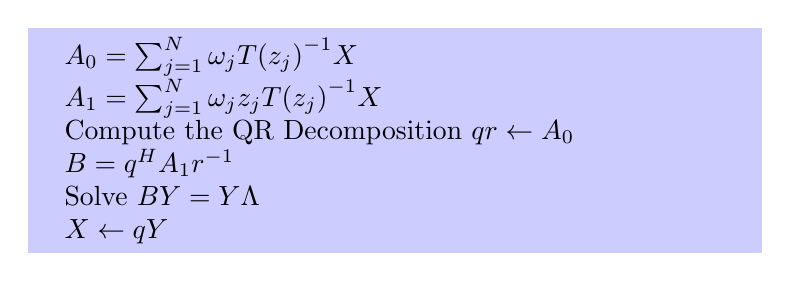
\begin{tikzpicture}
		\node[fill, color=blue,text=black, fill opacity=0.2, text opacity=1] {
		\begin{minipage}{0.75\linewidth}
			\begin{algorithmic}
	\STATE{\(A_0 = \sum_{j=1}^{N} \omega_j {T(z_j)}^{-1} X \)}
	\STATE{\(A_1 = \sum_{j=1}^{N} \omega_j z_j {T(z_j)}^{-1} X \)}
	\STATE{Compute the QR Decomposition \( qr \leftarrow A_0\)}
	\STATE{\( B = q^H A_1 r^{-1} \)}
	\STATE{Solve \( BY = Y \Lambda \)}
	\STATE{ \( X \leftarrow qY \)}
			\end{algorithmic}	
		\end{minipage}
		};
	\end{tikzpicture}
	\vspace{-1.5em}
	\begin{algorithmic}
	\WHILE{not converged}
\STATE{\(Q_0 \leftarrow \sum_{j=1}^{N} \omega_j [X - {T(z_j)}^{-1}T(X, \Lambda)] {(z_j I - \Lambda)}^{-1} \)}
\STATE{\(Q_1 \leftarrow \sum_{j=1}^{N} \omega_j z_j [X  - {T(z_j)}^{-1} T(X, \Lambda)] {(z_j I - \Lambda)}^{-1} \)}
	\STATE{Compute the QR Decomposition \( qr \leftarrow Q_0\)}
	\STATE{\( B \leftarrow q^H Q_1 r^{-1} \)}
	\STATE{Solve \( BY = Y \Lambda \)}
	\STATE{ \( X \leftarrow qY \)}
	\ENDWHILE
	\RETURN \( X, \Lambda \)
	\end{algorithmic}
\end{frame}

\begin{frame}{NLFEAST-Beyn Hybrid Algorithm}
	\begin{itemize}
		\item From one perspective, this can be viewed as NLFEAST using the decomposition of Beyn's method directly.

			No reduced system needs to be solved.

			\vspace{2em}
		\item From the other, it can be viewed as Beyn's method using the RII (from Neumaier) approach of NLFEAST.\@
			\vspace{2em}
		\item Can be reduced to standard FEAST for linear problems.
			\vspace{2em}
	\end{itemize}
\end{frame}



%%%%%%%%%%%%%%%%%%%%%%%%%%%%%%%%%%%%%%%%%%%%%%%%%%%%%%%%%%%%%%%%%%%%%%%%%%%%%%%%
\section{Experimental Results}
%%%%%%%%%%%%%%%%%%%%%%%%%%%%%%%%%%%%%%%%%%%%%%%%%%%%%%%%%%%%%%%%%%%%%%%%%%%%%%%%


\begin{frame}{Numerical Experiments}

    \centering Butterfly Problem (quartic)
    %\vspace{0.25em}

    \begin{figure}[htbp]
            \centering
	    \begin{tikzpicture}[scale=0.8]
            \begin{axis}[
                    ymode=log,
                    xmin=0.5,
                    xmax=13,
                    xtick=data,
                    unbounded coords=jump,
                    legend style={font=\tiny, fill opacity=0.9, row sep=-2.0},
		    legend image post style={scale=0.8},
                    xlabel={Iteration},
                    ymin=5.0e-17,
                    ylabel={Residual},
                    ymin=5.0e-17,
                    extra x ticks={1},
                    extra x tick labels={{\scriptsize(Beyn)}},
                    extra x tick style={{yshift=-2ex, grid=none}},
                    legend entries={\(N=8\), \(N=16\), \(N=32\), \(N=64\), \(N=128\), \(N=256\) } ]
                    %\addplot table [x=iter, y=$2$] {bf.dat};
                    \addplot table [x=iter, y=$3$] {bf.dat};
                    \addplot table [x=iter, y=$4$] {bf.dat};
                    \addplot table [x=iter, y=$5$] {bf.dat};
                    \addplot table [x=iter, y=$6$] {bf.dat};
                    \addplot table [x=iter, y=$7$] {bf.dat};
                    \addplot table [x=iter, y=$8$] {bf.dat};
                    \fill [blue, fill opacity=0.15] (0.5, 10.0) rectangle (1.5, 5.0e-17);
            \end{axis}
            \end{tikzpicture}
            \begin{tikzpicture}[scale=0.8]
            \begin{axis}[
                    xlabel={Real},
                    ylabel={Imaginary},
                    xmin=0,
                    xmax=2,
                    ymin=0,
                    ymax=2]
                    \draw [dashed, thick] (axis cs:1.0,1.0) circle [radius=0.5];
                    \addplot+ [only marks] table {bf_eig_in.dat};
                    \addplot+ [only marks, mark=*, mark options={solid, scale=0.35}] table {bf_eig.dat};
            \end{axis}
            \end{tikzpicture}
    \end{figure}

	\begin{table}
		\small
		\centering
		\begin{tabular}{lrr}
			\toprule
			\hspace{11em} & Linear System Solves & Factorizations \\
			\midrule
			\( N=16 \) & 208 & 16 \\
			\( N=32 \) & 160 & 32 \\
			\( N=64 \) & 192 & 64 \\
			\rowcolor{blue!10}
			Beyn       & 256 & 256 \\
			\bottomrule
		\end{tabular}
	\end{table}

    %208 linear system solves for \( N = 16 \).

    %192 solves for \( N = 32,64 \).

    %256 solves for Beyn.

    %Single precision / low accuracy solve.

  
\end{frame}


\begin{frame}{Numerical Experiments}
	\centering Hadeler Problem \hspace{1em} \( T(\lambda) = (e^\lambda - I)T_2 + \lambda^2 T_1 - \alpha T_0 \)
    %\vspace{0.25em}
    \begin{figure}[htbp]
            \centering
	    \begin{tikzpicture}[scale=0.8]
            \begin{axis}[
                    legend style={font=\tiny, fill opacity=0.9, row sep=-2.0},
		    legend image post style={scale=0.8},
                    unbounded coords=jump,
                    ymode=log,
                    xmax=10,
                    xmin=0.5,
                    xtick=data,
                    xlabel={Iteration},
                    ymin=1.0e-18,
                    ylabel={Residual},
                    extra x ticks={1},
                    extra x tick labels={{\scriptsize(Beyn)}},
                    extra x tick style={{yshift=-2ex, grid=none}},
                    legend entries={\(N=8\), \(N=16\), \(N=32\), \(N=64\), \(N=128\), \(N=256\) } ]
                    %\addplot table [x=iter, y=$2$] {hadeler.dat};
                    \addplot table [x=iter, y=$3$] {hadeler.dat};
                    \addplot table [x=iter, y=$4$] {hadeler.dat};
                    \addplot table [x=iter, y=$5$] {hadeler.dat};
                    \addplot table [x=iter, y=$6$] {hadeler.dat};
                    \addplot table [x=iter, y=$7$] {hadeler.dat};
                    \fill [blue, fill opacity=0.15] (0.5, 10.0) rectangle (1.5, 5.0e-19);
            \end{axis}
            \end{tikzpicture}
	    \begin{tikzpicture}[scale=0.8]
            \begin{axis}[
                    xlabel={Real},
                    ylabel={Imaginary},
                    xmin=-48,
                    xmax=-12,
                    ymin=-15,
                    ymax=15
                    ]
                    \draw[dashed, thick] (axis cs:-30.0,0.0) circle [radius=10.0];
                    \addplot+ [only marks] table {hadeler_eig_in.dat};
                    \addplot+ [only marks, mark=*, mark options={solid, scale=0.35}] table {hadeler_eig.dat};
            \end{axis}
            \end{tikzpicture}
    \end{figure}
    %144 solves for \( N = 16 \) contour points, only 16 factorizations!

    %160 solves for \( N = 32 \).

    %128 solves for \( N = 64 \).

    %More than 128 factorizations and solves for Beyn.

	\begin{table}
		\small
		\centering
		\begin{tabular}{lrr}
			\toprule
			\hspace{11em} & Linear System Solves & Factorizations \\
			\midrule
			\( N=16 \) & 144 & 16 \\
			\( N=32 \) & 160 & 32 \\
			\( N=64 \) & 128 & 64 \\
			\rowcolor{blue!10}
			Beyn       & \(\ge128\) & \(\ge128\) \\
			\bottomrule
		\end{tabular}
	\end{table}
\end{frame}

%%%%%%%%%%%%%%%%%%%%%%%%%%%%%%%%%%%%%%%%%%%%%%%%%%%%%%%%%%%%%%%%%
\section{Higher Moments}
\begin{frame}{Higher Moments}
	
	Necessary to use higher moments for eigenvector defects or many eigenvalues in a contour.

	\begin{align}
		H_0 = 
		\begin{bmatrix}
			{A}_0      & \cdots & {A}_{K-1}  \\
			\vdots             &        & \vdots \\
			{A}_{K-1}  & \cdots & {A}_{2K-2} 
		\end{bmatrix},
		H_1 = 
		\begin{bmatrix}
			{A}_1      & \cdots & {A}_{K}  \\
			\vdots             &        & \vdots \\
			{A}_{K}    & \cdots & {A}_{2K-1} 
		\end{bmatrix}.
	\end{align}

	\begin{align}
		V_{[K]} = 
		\begin{bmatrix}
			V \\
			\vdots \\
			V \Lambda^{K-1}
		\end{bmatrix},
		\quad
		W^H_{[K]} = \big[W^HX, \ldots, \Lambda^{K-1} W^H X \big]
	\end{align}
	
	Similar to the relation between \( A_0  \) and \( A_1 \) before
	\begin{align}
		H_0 = V_{[K]}W^H_{[K]}, \quad
		H_1 = V_{[K]} \Lambda W^H_{[K]}.
	\end{align}
	%General way of considering most higher moment algorithms by considering ``left probing matrix'' \( \widehat{X} \in \mathbb{C}^{n\times \ell} \) in addition to ``right probing matrix'' \( X \in \mathbb{C}^{n\times m} \) and defining
	%\begin{align}
		%\widehat{A}_k = \widehat{X}^H A_k
		%= \frac{1}{2 \pi i} \int_{\Gamma} z^k \widehat{X}^H {T(z)}^{-1} X \, dz.
	%\end{align}


\end{frame}

%\begin{frame}{Higher Moment Matrix}
	%Choosing \( K \in \mathbb{N} \) as the number of computed moments, form the \( K \ell \times K m \) block Hankel matrices
	%\begin{align}
		%H_0 = 
		%\begin{bmatrix}
			%\widehat{A}_0      & \cdots & \widehat{A}_{K-1}  \\
			%\vdots             &        & \vdots \\
			%\widehat{A}_{K-1}  & \cdots & \widehat{A}_{2K-2} 
		%\end{bmatrix},
		%H_1 = 
		%\begin{bmatrix}
			%\widehat{A}_1      & \cdots & \widehat{A}_{K}  \\
			%\vdots             &        & \vdots \\
			%\widehat{A}_{K}    & \cdots & \widehat{A}_{2K-1} 
		%\end{bmatrix}.
	%\end{align}
	%From the Keldysh theorem we have \( \widehat{A}_k = \widehat{X}V\Lambda^k W^H X \), letting
	%\begin{align}
		%V_{[K]} = 
		%\begin{bmatrix}
			%\widehat{X}V \\
			%\vdots \\
			%\widehat{X} V \Lambda^{K-1}
		%\end{bmatrix},
		%\quad
		%W^H_{[K]} = \big[W^HX, \ldots, \Lambda^{K-1} W^H X \big]
	%\end{align}
	%we have, similarly to before with \( A_0\) and \(A_1 \), that 
	%\begin{align}
		%H_0 = V_{[K]}W^H_{[K]}, \quad
		%H_1 = V_{[K]} \Lambda W^H_{[K]}.
	%\end{align}
%\end{frame}

%\begin{frame}{Higher Moment Methods}
	%Using the same similarity as Beyn's method, taking the SVD \( H_0 = V_0 \Sigma_0 W^H_0 \), we can diagonalize \( V_0^H H_1 W_0 \Sigma_0^{-1} \) to find \( \Lambda \).
	%Recovering the eigenvectors depends on the form of \( \widehat{X} \).
	%\vspace{1em}
	%\begin{itemize}
		%\item Taking \( \widehat{X} = I \in \mathbb{C}^{n \times n} \) gives Beyn's method.
			%\vspace{1em}
		%\item Taking \( \widehat{X} = X \) gives the SS-Hankel method.
			%Here \( H_0, H_1 \) are square and another approach is need to recover eigenvectors.

	%\end{itemize}

	%\vspace{1em}
	%For \( \widehat{X}=I \) (thus \( \widehat{A}_k = A_k \)) we have applied the RII method.
	%This requires deflating the subspace after every iteration.

%\end{frame}

\begin{frame}{Problems with Higher Moments}

	\begin{itemize}
		%\item Eigenvectors (potentially) only recoverable in special cases, limiting iteration to Beyn and SS type methods.
			%\vspace{1em}
		\item SS-Hankel approach has benefits, but not yet explored.
			\vspace{2em}
		\item Deflation after every iteration limits number of eigenvalues. Unclear how RII can be modified to reuse all spectral information after iteration (work in progress).
			%\vspace{1em}
		%\item No easy way to determine when there are deficient eigenvectors without computing many higher moments.
			%\vspace{1em}
		
	\end{itemize}

	
\end{frame}

\section{Conclusion}

\begin{frame}{Future Work}
	\begin{itemize}
		\item Higher moments.
		\vspace{1em}
		\item Analysis of contour shifted RII.
		\vspace{1em}
		\item Theoretical relation to other algorithms.
	\end{itemize}
\end{frame}

\begin{frame}{Software}
	\begin{itemize}
		\item The \href{http://http://www.ecs.umass.edu/~polizzi/feast/}{FEAST library} 
			\vspace{0.5em}
			\begin{itemize}
				\item Polynomial solver in FEAST 4.0 (current release).
					\vspace{0.5em}
				\item Hybrid (fully nonlinear) solver in FEAST 5.0 (upcoming).
			\end{itemize}
		\vspace{1em}
	\item \href{https://github.com/spacedome/FEASTSolver.jl}{FEASTSolver.jl} (used in numerical results)
		\vspace{0.5em}
		\begin{itemize}
			\item Julia implementation.
				\vspace{0.5em}
			\item Less optimized, very extensible, fully nonlinear.
				\vspace{0.5em}
			\item Will (eventually) be compatible with NEP-PACK.
		\end{itemize}
		\vspace{1em}
		\item FEAST.jl Julia bindings (work in progress!)
	\end{itemize}
\end{frame}

\begin{frame}{Citations}
	\bibliography{references}
	\bibliographystyle{unsrt}
\end{frame}

\end{document}
